\documentclass[12pt,a4paper,openany]{book}

\input{C:/Users/serru/Documents/Codes/LaTeX/Environnement_package.tex}
\input{C:/Users/serru/Documents/Codes/LaTeX/Environnements_settings.tex}
\input{C:/Users/serru/Documents/Codes/LaTeX/Environnement_theorems.tex}

\setcounter{tocdepth}{4}
\sloppy

\title{}
\author{Serrurot Gabin\\
BTS SNIR}
\date{\today}

\begin{document}

\sloppy

\vspace*{\stretch{1}}
\begin{minipage}{0.9\linewidth}
\rule{\linewidth}{0.5mm}\\[0.2cm]
\huge\bfseries
\begin{center}
Mathématiques
\end{center}
\rule{\linewidth}{0.5mm}\\[0.2cm]
\maketitle
\end{minipage}
\vspace*{\stretch{1}}

\newpage

\tableofcontents

\newpage

\chapter{Trigonométrie}

\section{Cercle trigonométrique}

\begin{figure}[!h]
\begin{center}
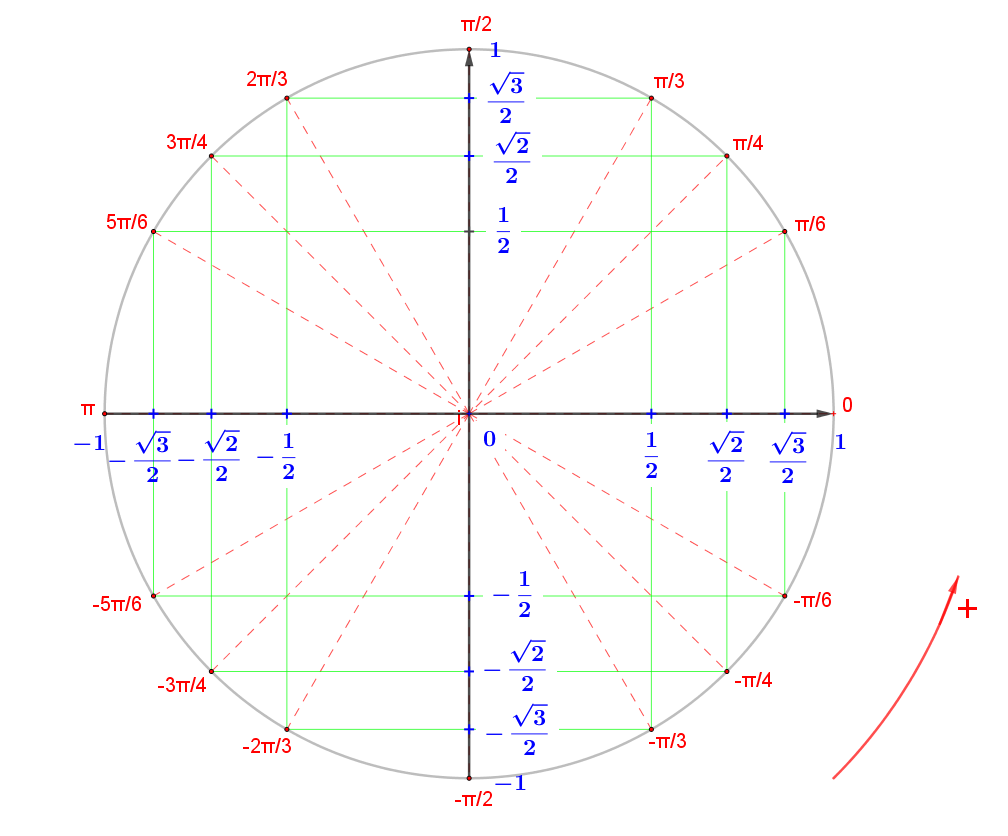
\includegraphics[scale=0.5]{Images/cercleTrigonometrique.png} 
\caption{Image montrant le cercle trigonométrique.}
\label{cercleTrigo}
\end{center}
\end{figure}

\section{Fonctions sinus et cosinus}

\paragraph{Cosinus} Nous avons plusieurs relations remarquables pour la fonction $ cos(x) $:
\begin{align}
cos(x) & = cos(-x)\\
cos(\pi - x) & = -cos(x) = cos(\pi + x)
\end{align}

Nous pouvons associer à cette fonction la fonction \textbf{$ arccos(x) $} qui est sa \textbf{fonction réciproque}. Elle est définie sur $ [0; \pi] $.

\paragraph{Sinus} Nous avons plusieurs relations remarquables pour la fonction $ sin(x) $:
\begin{align}
sin(x) & = -sin(x)\\
sin(\pi - x) & = sin(x)\\
sin(\pi + x) & = -sin(x)
\end{align}

Nous pouvons associer à cette fonction la fonction \textbf{$ arcsin(x) $} qui est sa \textbf{fonction réciproque}. Elle est définie sur $ [-\frac{\pi}{2}; \frac{\pi}{2}] $.

\section{Fonction tangente}

On peut définir la tangente comme étant le \textbf{rapport} du \textbf{sinus} et du \textbf{cosinus}. Elle est définie sur $ ]-\frac{\pi}{2}; \frac{\pi}{2}[ $.\\
Nous avons donc sa représentation graphique suivante:
\begin{figure}[!h]
\begin{center}
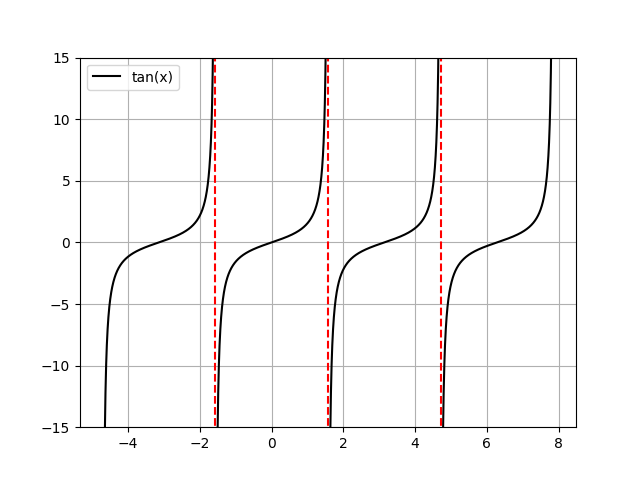
\includegraphics[scale=0.8]{Images/grapheTan.png} 
\caption{graphique représentant l'allure de la fonction tangente.}
\label{grapheTan}
\end{center}
\end{figure}

\newpage

Ses valeurs remarquables sont:
\begin{table}[!h]
\begin{center}
\begin{tabular}{|c|c|c|c|c|c|} %c/l/r pour centré/à gauche/droite
\hline $ x $ & $ 0 $ & $ \dfrac{\pi}{6} $ & $ \dfrac{\pi}{4} $ & $ \dfrac{\pi}{3} $ & $ \dfrac{\pi}{2} $\\
\hline $ tan(x) $ & $ 0 $ & $ \dfrac{1}{\sqrt{3}} $ & $ 1 $ & $ \sqrt{3} $ & interdit\\
\hline
\end{tabular}
\caption{Tableau montrant les valeurs remarquables de la fonction $ tan(x) $.}
\label{tableauValeursTangente}
\end{center}
\end{table}

Nous avons donc les propriétés suivantes:
\begin{align}
tan(-x) & = -tan(x)\\
tan(\pi - x) & = -tan(x)\\
tan(\pi + x) & = tan(x)
\end{align}

Nous pouvons associer à la fonction tangente une \textbf{fonction réciproque}, la fonction \textbf{$ arctan(x) $} dont la représentation est dans la figure ci-dessous:
\begin{figure}[!h]
\begin{center}
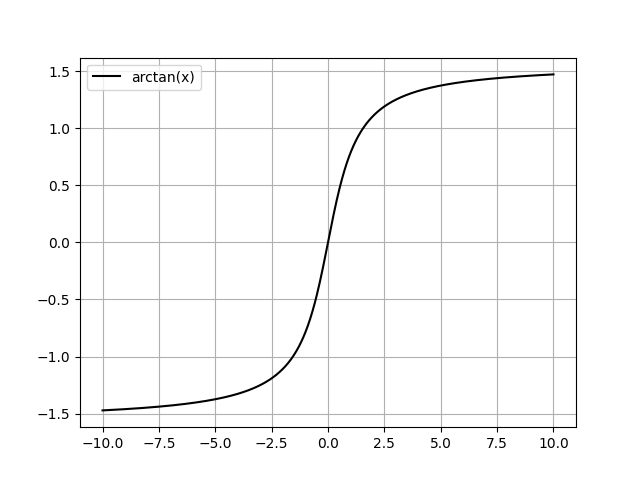
\includegraphics[scale=0.8]{Images/grapheArctan.png} 
\caption{Graphique montrant l'allure de la fonction $ arctan(x) $.}
\label{grapheArctan}
\end{center}

Nous pouvons associer à cette fonction réciproque la relation:
\begin{equation}
arctan(-x) = -arctan(x)
\end{equation}
\end{figure}

\chapter{Généralités sur les fonctions usuelles}

\section{Fonctions usuelles}

Les fonctions usuelles sont représentées sur le graphe ci-dessous:
\begin{figure}[!h]
\begin{center}
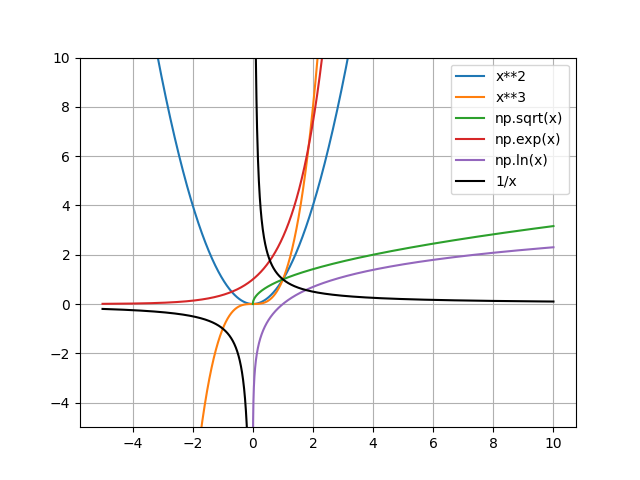
\includegraphics[scale=0.8]{Images/grapheFonctionsRemarquables.png} 
\caption{Graphique montrant les fonctions usuelles.}
\label{grapheFonctionsUsuelles}
\end{center}
\end{figure}

\section{Dérivées de fonctions usuelles}

Le nombre dérivé d'une fonction \textbf{en un point} représente le \textbf{coefficient directeur} de la tangente en ce point. En effet, en chaque point nous pouvons tracer une droite qui \textbf{"colle"} à la courbe. On trouve ainsi une droite de la forme \textbf{$ y = ax + b $} dont le coefficient directeur est le nombre dérivé en ce point. Le nombre dérivé en a est noté \textbf{$ f'(a) $}. En calculant le nombre dérivé pour \textbf{chacun des points} de la fonction, on obtient la \textbf{fonction dérivée}. En réalité, l'équation d'une tangente est de la forme:
\begin{equation}
y = f'(a)(x - a) + f(a)
\end{equation}

\section{Calculer une dérivée de fonctions usuelles}

Nous pouvons dresser le tableau qui donne les dérivées de chaque fonction usuelle:
\begin{table}[!h]
\begin{center}
\begin{tabular}{|c|c|c|c|c|c|} %c/l/r pour centré/à gauche/droite
\hline $ f(x) $ & $ k $ & $ x^{n} $ & $ \dfrac{1}{x} $ & $ \sqrt{x} $ & $ e^{x} $\\
\hline $ f'(x) $ & $ 0 $ & $ nx^{n-1} $ & $ -\dfrac{1}{x^{2}} $ & $ \dfrac{1}{2\sqrt{x}} $ & $ e^{x} $\\
\hline
\end{tabular}
\caption{Tableau montrant la forme des dérivées des fonctions usuelles.}
\label{tableauDeriveesUsuelles}
\end{center}
\end{table}

De plus, si nous avons la dérivée de fonctions usuelles avec une opération entre elles, nous avons les relations suivantes:
\begin{table}[!h]
\begin{center}
\begin{tabular}{|c|c|c|c|c|c|c|} %c/l/r pour centré/à gauche/droite
\hline $ f(x) $ & $ u(x) + v(x) $ & $ u(x)v(x) $ & $ ku(x) $ & $ \dfrac{u(x)}{v(x)} $ & $ \dfrac{k}{u(x)} $ & $ \dfrac{u(x)}{k} $\\
\hline $ f'(x) $ & $ u'(x) + v'(x) $ & $ u'(x)v(x) + u(x)v'(x) $ & $ ku'(x) $ & $ \dfrac{u'(x)v(x) - u(x)v'(x)}{v^{2}(x)} $ & $ -\dfrac{ku'(x)}{u^{2}(x)} $ & $ \dfrac{u'(x)}{k} $\\
\hline
\end{tabular}
\caption{Forme des dérivées de fonctions usuelles.}
\label{tableauDeriveesFonctionsUsuelles}
\end{center}
\end{table}

Nous pouvons utiliser la notion de \textbf{dérivabilité} pour déduire le \textbf{nombre de solutions} d'une équation lorsque celle-ci n'est pas soluble. Ainsi, si nous avons:
\begin{enumerate}
\item $ f $ est dérivable et de variation strictement identique sur un intervalle $ I $
\item $ k $ est un réel faisant partie de l'ensemble des images des réels parcourant $ I $
\end{enumerate}

alors, l'équation $ f(x) = k $ admet une unique solution sur l'intervalle $ I $.

\chapter{Nombres complexes}

\section{Définir et représenter un nombre complexe}

Un nombre complexe peut s'écrire $ z = a + ib $. Cette représentation s'appelle \textbf{forme algébrique} ou \textbf{forme cartésienne}. Un nombre complexe est donc composé d'une partie réelle (ici $ \mathfrak{Re}(z) = a $) et d'une partie imaginaire (ici $ \mathfrak{Im}(z) = b $). Nous pouvons noter que si $ a = 0 $, alors $ z $ est un \textbf{imaginaire pur}. Si $ b = 0 $, alors $ z $ est un \textbf{nombre réel}.\\

Puisqu'un \textbf{réel} est représenté sur une droite (la \textbf{droite des réels}), un \textbf{nombre complexe} se représente dans le \textbf{plan complexe}.

!!!	INSERER A L'OCCASION UN GRAPHE D'UN NOMBRE COMPLEXE !!!

\section{Calculs avec les complexes}

Si nous \textbf{n'avons pas} de division de complexes, alors pour réaliser les autres opérations il faut juste \textbf{remplacer} le nombre en mettant les \textbf{parenthèses}. Par exemple, si nous avons $ z_{1} = 2 - 3i $ et $ z_{2} = 1 + 4i $, alors le produit des deux donne:
\begin{align*}
z_{1}.z_{2} & = (2 - 3i).(1 + 4i)\\
		   & = 2 + 8i - 3i -12i^{2}\\
		   & = 2 + 5i + 12 \text{\hspace{50px} car $ i^{2} = -1 $}\\
		   & = 14 + 5i
\end{align*}

Nous pouvons introduire la notion de \textbf{complexe conjugué}. Il s'agit du complexe ayant la \textbf{même partie réelle} mais avec une \textbf{partie imaginaire opposée}. Par exemple, $ z_{1} = 2 - 3i $ a pour conjugué $ \overline{z_{1}} = 2 + 3i $. Nous avons donc la relation suivante:
\begin{equation}
z\overline{z} = a^{2} + b^{2}
\end{equation}

Cependant, si nous avons un \textbf{quotient} dans le calcul, alors nous devons \textbf{multiplier} au \textbf{numérateur et au dénominateur} par le complexe \textbf{conjugué} du \textbf{dénominateur}. Par exemple:
\begin{align*}
\dfrac{2 - 3i}{1 + 4i} & = \dfrac{(2 - 3i).(1 - 4i}{(1 + 4i).(1 - 4i)}\\
					   & = \dfrac{2 - 8i - 3i - 12i^{2}}{17}\\
					   & = \dfrac{14 - 11i}{17}\\
					   & = \dfrac{14}{17} - \dfrac{11}{17}i
\end{align*}

\section{Forme trigonométrique d'un nombre complexe}

Lorsqu'un nombre complexe est représenté dans le plan complexe, il forme alors un \textbf{triangle rectangle} de côtés $ a $ et $ b $. L'\textbf{hypoténuse} de ce triangle rectangle s'appelle le \textbf{module} de $ z $ et se note $ |z| = r $ tandis que l'angle qui est \textbf{opposé} à $ b $ s'appelle l'\textbf{argument} et se note $ arg(z) = \theta $.\\
Pour calculer le module, nous avons:
\begin{equation}
|z| = r = \sqrt{a^{2} + b^{2}}
\end{equation}

Pour calculer l'argument, nous avons:
\begin{align}
arg(z) & = \theta = arctan(\dfrac{b}{a}) \text{\hspace{50px} si $ a > 0 $}\\
arg(z) & = \theta = arctan(\dfrac{b}{a}) + \pi \text{\hspace{30px} si $ a < 0 $}
\end{align}

Avec tout ceci, en utilisant \textbf{SoCaTo}, nous trouvons que $ a = rcos(\theta) $ et $ b = rsin(\theta) $. Ainsi, nous avons:
\begin{equation}
z = a + ib = r(cos(\theta) + isin(\theta))
\end{equation}

Cette manière d'écrire un nombre complexe s'appelle la \textbf{forme trigonométrique} et peut se noter de manière simplifiée $ z = [r, \theta] $. Nous pouvons noter que par identification entre la forme algébrique et la forme trigonométrique, nous avons:
\begin{align*}
|r| & = \sqrt{a^{2} + b^{2}}\\
\theta & = arctan(\dfrac{b}{a}) \text{\hspace{50px} si $ a > 0 $}\\
	   & = arctan(\dfrac{b}{a}) + \pi \text{\hspace{30px} si $ a < 0 $}\\
a & = |r|cos(\theta)\\
b & = |r|sin(\theta)
\end{align*}

Nous avons des relations remarquables sur le module et l'argument d'un nombre complexe:
\begin{align}
|zz'| & = |z|.|z'| \text{\hspace{40px} et \hspace{40px}} arg(zz') = arg(z) + arg(z')\\
|\dfrac{z}{z'}| & = \dfrac{|z|}{|z'|} \text{\hspace{55px} et \hspace{40px}} arg(\dfrac{z}{z'}) = arg(z) - arg(z')
\end{align}

\section{Racines complexes d'un polynôme du second degré à coefficients réels}

\end{document}